% Created by tikzDevice version 0.12.6 on 2024-02-29 10:34:59
% !TEX encoding = UTF-8 Unicode
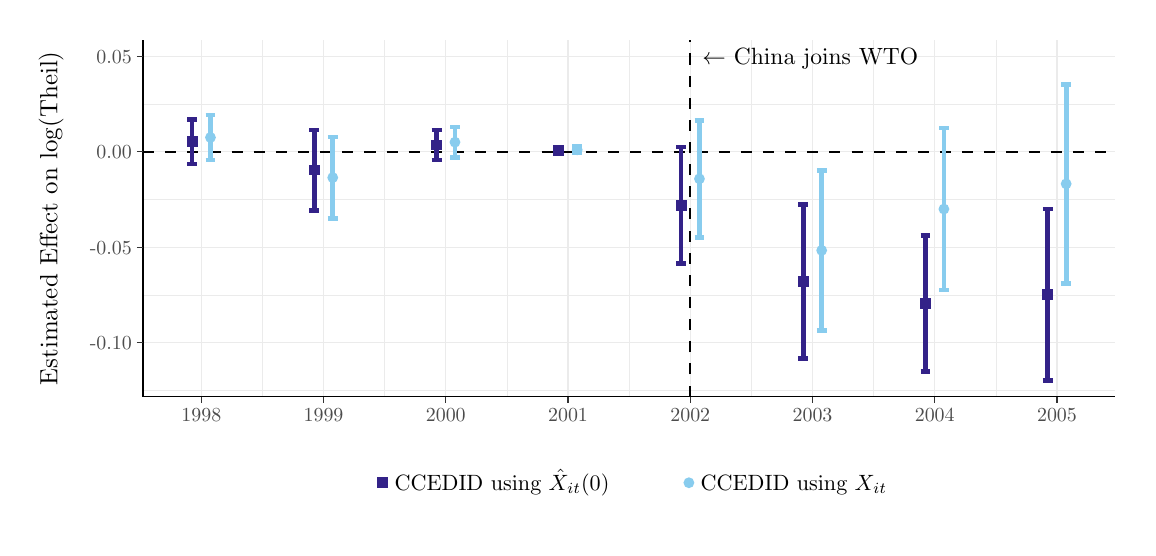
\begin{tikzpicture}[x=1pt,y=1pt]
\definecolor{fillColor}{RGB}{255,255,255}
\path[use as bounding box,fill=fillColor] (0,0) rectangle (397.48,180.67);
\begin{scope}
\path[clip] (  0.00,  0.00) rectangle (397.48,180.67);
\definecolor{drawColor}{RGB}{255,255,255}

\path[draw=drawColor,line width= 0.5pt,line join=round,line cap=round,fill=fillColor] (  0.00,  0.00) rectangle (397.48,180.68);
\end{scope}
\begin{scope}
\path[clip] ( 41.69, 47.36) rectangle (392.98,176.17);
\definecolor{fillColor}{RGB}{255,255,255}

\path[fill=fillColor] ( 41.69, 47.36) rectangle (392.98,176.17);
\definecolor{drawColor}{gray}{0.92}

\path[draw=drawColor,line width= 0.2pt,line join=round] ( 41.69, 49.60) --
	(392.98, 49.60);

\path[draw=drawColor,line width= 0.2pt,line join=round] ( 41.69, 84.09) --
	(392.98, 84.09);

\path[draw=drawColor,line width= 0.2pt,line join=round] ( 41.69,118.58) --
	(392.98,118.58);

\path[draw=drawColor,line width= 0.2pt,line join=round] ( 41.69,153.07) --
	(392.98,153.07);

\path[draw=drawColor,line width= 0.2pt,line join=round] ( 84.83, 47.36) --
	( 84.83,176.17);

\path[draw=drawColor,line width= 0.2pt,line join=round] (129.00, 47.36) --
	(129.00,176.17);

\path[draw=drawColor,line width= 0.2pt,line join=round] (173.17, 47.36) --
	(173.17,176.17);

\path[draw=drawColor,line width= 0.2pt,line join=round] (217.34, 47.36) --
	(217.34,176.17);

\path[draw=drawColor,line width= 0.2pt,line join=round] (261.51, 47.36) --
	(261.51,176.17);

\path[draw=drawColor,line width= 0.2pt,line join=round] (305.68, 47.36) --
	(305.68,176.17);

\path[draw=drawColor,line width= 0.2pt,line join=round] (349.85, 47.36) --
	(349.85,176.17);

\path[draw=drawColor,line width= 0.5pt,line join=round] ( 41.69, 66.85) --
	(392.98, 66.85);

\path[draw=drawColor,line width= 0.5pt,line join=round] ( 41.69,101.34) --
	(392.98,101.34);

\path[draw=drawColor,line width= 0.5pt,line join=round] ( 41.69,135.83) --
	(392.98,135.83);

\path[draw=drawColor,line width= 0.5pt,line join=round] ( 41.69,170.32) --
	(392.98,170.32);

\path[draw=drawColor,line width= 0.5pt,line join=round] ( 62.74, 47.36) --
	( 62.74,176.17);

\path[draw=drawColor,line width= 0.5pt,line join=round] (106.91, 47.36) --
	(106.91,176.17);

\path[draw=drawColor,line width= 0.5pt,line join=round] (151.08, 47.36) --
	(151.08,176.17);

\path[draw=drawColor,line width= 0.5pt,line join=round] (195.25, 47.36) --
	(195.25,176.17);

\path[draw=drawColor,line width= 0.5pt,line join=round] (239.43, 47.36) --
	(239.43,176.17);

\path[draw=drawColor,line width= 0.5pt,line join=round] (283.60, 47.36) --
	(283.60,176.17);

\path[draw=drawColor,line width= 0.5pt,line join=round] (327.77, 47.36) --
	(327.77,176.17);

\path[draw=drawColor,line width= 0.5pt,line join=round] (371.94, 47.36) --
	(371.94,176.17);
\definecolor{drawColor}{RGB}{0,0,0}

\path[draw=drawColor,line width= 0.6pt,dash pattern=on 4pt off 4pt ,line join=round] ( 41.69,135.83) -- (392.98,135.83);

\path[draw=drawColor,line width= 0.6pt,dash pattern=on 4pt off 4pt ,line join=round] (239.43, 47.36) -- (239.43,176.17);

\node[text=drawColor,anchor=base west,inner sep=0pt, outer sep=0pt, scale=  0.85] at (243.84,167.38) {$\leftarrow$ China joins WTO};
\definecolor{drawColor}{RGB}{51,34,136}

\path[draw=drawColor,line width= 1.7pt,line join=round] ( 57.66,147.51) --
	( 61.20,147.51);

\path[draw=drawColor,line width= 1.7pt,line join=round] ( 59.43,147.51) --
	( 59.43,131.45);

\path[draw=drawColor,line width= 1.7pt,line join=round] ( 57.66,131.45) --
	( 61.20,131.45);

\path[draw=drawColor,line width= 1.7pt,line join=round] (101.83,143.74) --
	(105.37,143.74);

\path[draw=drawColor,line width= 1.7pt,line join=round] (103.60,143.74) --
	(103.60,114.71);

\path[draw=drawColor,line width= 1.7pt,line join=round] (101.83,114.71) --
	(105.37,114.71);

\path[draw=drawColor,line width= 1.7pt,line join=round] (146.00,143.67) --
	(149.54,143.67);

\path[draw=drawColor,line width= 1.7pt,line join=round] (147.77,143.67) --
	(147.77,132.89);

\path[draw=drawColor,line width= 1.7pt,line join=round] (146.00,132.89) --
	(149.54,132.89);

\path[draw=drawColor,line width= 1.7pt,line join=round] (190.17,137.42) --
	(193.71,137.42);

\path[draw=drawColor,line width= 1.7pt,line join=round] (191.94,137.42) --
	(191.94,135.23);

\path[draw=drawColor,line width= 1.7pt,line join=round] (190.17,135.23) --
	(193.71,135.23);

\path[draw=drawColor,line width= 1.7pt,line join=round] (234.35,137.52) --
	(237.88,137.52);

\path[draw=drawColor,line width= 1.7pt,line join=round] (236.11,137.52) --
	(236.11, 95.43);

\path[draw=drawColor,line width= 1.7pt,line join=round] (234.35, 95.43) --
	(237.88, 95.43);

\path[draw=drawColor,line width= 1.7pt,line join=round] (278.52,116.79) --
	(282.05,116.79);

\path[draw=drawColor,line width= 1.7pt,line join=round] (280.28,116.79) --
	(280.28, 61.09);

\path[draw=drawColor,line width= 1.7pt,line join=round] (278.52, 61.09) --
	(282.05, 61.09);

\path[draw=drawColor,line width= 1.7pt,line join=round] (322.69,105.68) --
	(326.22,105.68);

\path[draw=drawColor,line width= 1.7pt,line join=round] (324.45,105.68) --
	(324.45, 56.47);

\path[draw=drawColor,line width= 1.7pt,line join=round] (322.69, 56.47) --
	(326.22, 56.47);

\path[draw=drawColor,line width= 1.7pt,line join=round] (366.86,115.16) --
	(370.39,115.16);

\path[draw=drawColor,line width= 1.7pt,line join=round] (368.62,115.16) --
	(368.62, 53.22);

\path[draw=drawColor,line width= 1.7pt,line join=round] (366.86, 53.22) --
	(370.39, 53.22);
\definecolor{drawColor}{RGB}{136,204,238}

\path[draw=drawColor,line width= 1.7pt,line join=round] ( 64.29,149.12) --
	( 67.82,149.12);

\path[draw=drawColor,line width= 1.7pt,line join=round] ( 66.05,149.12) --
	( 66.05,132.86);

\path[draw=drawColor,line width= 1.7pt,line join=round] ( 64.29,132.86) --
	( 67.82,132.86);

\path[draw=drawColor,line width= 1.7pt,line join=round] (108.46,141.19) --
	(111.99,141.19);

\path[draw=drawColor,line width= 1.7pt,line join=round] (110.23,141.19) --
	(110.23,111.81);

\path[draw=drawColor,line width= 1.7pt,line join=round] (108.46,111.81) --
	(111.99,111.81);

\path[draw=drawColor,line width= 1.7pt,line join=round] (152.63,144.75) --
	(156.16,144.75);

\path[draw=drawColor,line width= 1.7pt,line join=round] (154.40,144.75) --
	(154.40,133.84);

\path[draw=drawColor,line width= 1.7pt,line join=round] (152.63,133.84) --
	(156.16,133.84);

\path[draw=drawColor,line width= 1.7pt,line join=round] (196.80,137.64) --
	(200.33,137.64);

\path[draw=drawColor,line width= 1.7pt,line join=round] (198.57,137.64) --
	(198.57,135.43);

\path[draw=drawColor,line width= 1.7pt,line join=round] (196.80,135.43) --
	(200.33,135.43);

\path[draw=drawColor,line width= 1.7pt,line join=round] (240.97,147.22) --
	(244.50,147.22);

\path[draw=drawColor,line width= 1.7pt,line join=round] (242.74,147.22) --
	(242.74,104.89);

\path[draw=drawColor,line width= 1.7pt,line join=round] (240.97,104.89) --
	(244.50,104.89);

\path[draw=drawColor,line width= 1.7pt,line join=round] (285.14,129.17) --
	(288.68,129.17);

\path[draw=drawColor,line width= 1.7pt,line join=round] (286.91,129.17) --
	(286.91, 71.23);

\path[draw=drawColor,line width= 1.7pt,line join=round] (285.14, 71.23) --
	(288.68, 71.23);

\path[draw=drawColor,line width= 1.7pt,line join=round] (329.31,144.39) --
	(332.85,144.39);

\path[draw=drawColor,line width= 1.7pt,line join=round] (331.08,144.39) --
	(331.08, 85.86);

\path[draw=drawColor,line width= 1.7pt,line join=round] (329.31, 85.86) --
	(332.85, 85.86);

\path[draw=drawColor,line width= 1.7pt,line join=round] (373.48,160.23) --
	(377.02,160.23);

\path[draw=drawColor,line width= 1.7pt,line join=round] (375.25,160.23) --
	(375.25, 88.25);

\path[draw=drawColor,line width= 1.7pt,line join=round] (373.48, 88.25) --
	(377.02, 88.25);
\definecolor{fillColor}{RGB}{51,34,136}

\path[fill=fillColor] ( 57.47,137.52) --
	( 61.39,137.52) --
	( 61.39,141.45) --
	( 57.47,141.45) --
	cycle;

\path[fill=fillColor] (101.64,127.26) --
	(105.56,127.26) --
	(105.56,131.19) --
	(101.64,131.19) --
	cycle;

\path[fill=fillColor] (145.81,136.32) --
	(149.73,136.32) --
	(149.73,140.24) --
	(145.81,140.24) --
	cycle;

\path[fill=fillColor] (189.98,134.37) --
	(193.90,134.37) --
	(193.90,138.29) --
	(189.98,138.29) --
	cycle;

\path[fill=fillColor] (234.15,114.51) --
	(238.07,114.51) --
	(238.07,118.44) --
	(234.15,118.44) --
	cycle;

\path[fill=fillColor] (278.32, 86.98) --
	(282.25, 86.98) --
	(282.25, 90.90) --
	(278.32, 90.90) --
	cycle;

\path[fill=fillColor] (322.49, 79.11) --
	(326.42, 79.11) --
	(326.42, 83.04) --
	(322.49, 83.04) --
	cycle;

\path[fill=fillColor] (366.66, 82.23) --
	(370.59, 82.23) --
	(370.59, 86.15) --
	(366.66, 86.15) --
	cycle;
\definecolor{fillColor}{RGB}{136,204,238}

\path[fill=fillColor] ( 66.05,140.99) circle (  1.96);

\path[fill=fillColor] (110.23,126.50) circle (  1.96);

\path[fill=fillColor] (154.40,139.29) circle (  1.96);

\path[fill=fillColor] (198.57,136.53) circle (  1.96);

\path[fill=fillColor] (242.74,126.05) circle (  1.96);

\path[fill=fillColor] (286.91,100.20) circle (  1.96);

\path[fill=fillColor] (331.08,115.13) circle (  1.96);

\path[fill=fillColor] (375.25,124.24) circle (  1.96);
\end{scope}
\begin{scope}
\path[clip] (  0.00,  0.00) rectangle (397.48,180.67);
\definecolor{drawColor}{RGB}{0,0,0}

\path[draw=drawColor,line width= 0.5pt,line join=round] ( 41.69, 47.36) --
	( 41.69,176.17);
\end{scope}
\begin{scope}
\path[clip] (  0.00,  0.00) rectangle (397.48,180.67);
\definecolor{drawColor}{gray}{0.30}

\node[text=drawColor,anchor=base east,inner sep=0pt, outer sep=0pt, scale=  0.72] at ( 37.64, 64.37) {-0.10};

\node[text=drawColor,anchor=base east,inner sep=0pt, outer sep=0pt, scale=  0.72] at ( 37.64, 98.86) {-0.05};

\node[text=drawColor,anchor=base east,inner sep=0pt, outer sep=0pt, scale=  0.72] at ( 37.64,133.35) {0.00};

\node[text=drawColor,anchor=base east,inner sep=0pt, outer sep=0pt, scale=  0.72] at ( 37.64,167.84) {0.05};
\end{scope}
\begin{scope}
\path[clip] (  0.00,  0.00) rectangle (397.48,180.67);
\definecolor{drawColor}{gray}{0.20}

\path[draw=drawColor,line width= 0.5pt,line join=round] ( 39.44, 66.85) --
	( 41.69, 66.85);

\path[draw=drawColor,line width= 0.5pt,line join=round] ( 39.44,101.34) --
	( 41.69,101.34);

\path[draw=drawColor,line width= 0.5pt,line join=round] ( 39.44,135.83) --
	( 41.69,135.83);

\path[draw=drawColor,line width= 0.5pt,line join=round] ( 39.44,170.32) --
	( 41.69,170.32);
\end{scope}
\begin{scope}
\path[clip] (  0.00,  0.00) rectangle (397.48,180.67);
\definecolor{drawColor}{RGB}{0,0,0}

\path[draw=drawColor,line width= 0.5pt,line join=round] ( 41.69, 47.36) --
	(392.98, 47.36);
\end{scope}
\begin{scope}
\path[clip] (  0.00,  0.00) rectangle (397.48,180.67);
\definecolor{drawColor}{gray}{0.20}

\path[draw=drawColor,line width= 0.5pt,line join=round] ( 62.74, 45.11) --
	( 62.74, 47.36);

\path[draw=drawColor,line width= 0.5pt,line join=round] (106.91, 45.11) --
	(106.91, 47.36);

\path[draw=drawColor,line width= 0.5pt,line join=round] (151.08, 45.11) --
	(151.08, 47.36);

\path[draw=drawColor,line width= 0.5pt,line join=round] (195.25, 45.11) --
	(195.25, 47.36);

\path[draw=drawColor,line width= 0.5pt,line join=round] (239.43, 45.11) --
	(239.43, 47.36);

\path[draw=drawColor,line width= 0.5pt,line join=round] (283.60, 45.11) --
	(283.60, 47.36);

\path[draw=drawColor,line width= 0.5pt,line join=round] (327.77, 45.11) --
	(327.77, 47.36);

\path[draw=drawColor,line width= 0.5pt,line join=round] (371.94, 45.11) --
	(371.94, 47.36);
\end{scope}
\begin{scope}
\path[clip] (  0.00,  0.00) rectangle (397.48,180.67);
\definecolor{drawColor}{gray}{0.30}

\node[text=drawColor,anchor=base,inner sep=0pt, outer sep=0pt, scale=  0.72] at ( 62.74, 38.35) {1998};

\node[text=drawColor,anchor=base,inner sep=0pt, outer sep=0pt, scale=  0.72] at (106.91, 38.35) {1999};

\node[text=drawColor,anchor=base,inner sep=0pt, outer sep=0pt, scale=  0.72] at (151.08, 38.35) {2000};

\node[text=drawColor,anchor=base,inner sep=0pt, outer sep=0pt, scale=  0.72] at (195.25, 38.35) {2001};

\node[text=drawColor,anchor=base,inner sep=0pt, outer sep=0pt, scale=  0.72] at (239.43, 38.35) {2002};

\node[text=drawColor,anchor=base,inner sep=0pt, outer sep=0pt, scale=  0.72] at (283.60, 38.35) {2003};

\node[text=drawColor,anchor=base,inner sep=0pt, outer sep=0pt, scale=  0.72] at (327.77, 38.35) {2004};

\node[text=drawColor,anchor=base,inner sep=0pt, outer sep=0pt, scale=  0.72] at (371.94, 38.35) {2005};
\end{scope}
\begin{scope}
\path[clip] (  0.00,  0.00) rectangle (397.48,180.67);
\definecolor{drawColor}{RGB}{0,0,0}

\node[text=drawColor,rotate= 90.00,anchor=base,inner sep=0pt, outer sep=0pt, scale=  0.90] at ( 10.70,111.77) {Estimated Effect on $\log($Theil$)$};
\end{scope}
\begin{scope}
\path[clip] (  0.00,  0.00) rectangle (397.48,180.67);
\definecolor{fillColor}{RGB}{255,255,255}

\path[fill=fillColor] (109.62,  4.50) rectangle (325.06, 27.95);
\end{scope}
\begin{scope}
\path[clip] (  0.00,  0.00) rectangle (397.48,180.67);
\definecolor{fillColor}{RGB}{255,255,255}

\path[fill=fillColor] (114.12,  9.00) rectangle (142.57, 23.45);
\end{scope}
\begin{scope}
\path[clip] (  0.00,  0.00) rectangle (397.48,180.67);
\definecolor{fillColor}{RGB}{51,34,136}

\path[fill=fillColor] (126.38, 14.26) --
	(130.31, 14.26) --
	(130.31, 18.19) --
	(126.38, 18.19) --
	cycle;
\end{scope}
\begin{scope}
\path[clip] (  0.00,  0.00) rectangle (397.48,180.67);
\definecolor{fillColor}{RGB}{255,255,255}

\path[fill=fillColor] (224.70,  9.00) rectangle (253.15, 23.45);
\end{scope}
\begin{scope}
\path[clip] (  0.00,  0.00) rectangle (397.48,180.67);
\definecolor{fillColor}{RGB}{136,204,238}

\path[fill=fillColor] (238.93, 16.23) circle (  1.96);
\end{scope}
\begin{scope}
\path[clip] (  0.00,  0.00) rectangle (397.48,180.67);
\definecolor{drawColor}{RGB}{0,0,0}

\node[text=drawColor,anchor=base west,inner sep=0pt, outer sep=0pt, scale=  0.80] at (132.57, 13.47) {CCEDID using $\hat{X}_{it}(0)$};
\end{scope}
\begin{scope}
\path[clip] (  0.00,  0.00) rectangle (397.48,180.67);
\definecolor{drawColor}{RGB}{0,0,0}

\node[text=drawColor,anchor=base west,inner sep=0pt, outer sep=0pt, scale=  0.80] at (243.15, 13.47) {CCEDID using $X_{it}$};
\end{scope}
\end{tikzpicture}
